\section{Results}
\label{sec:results}

%% Sections 4.1--4.3 report measurements that already exist and are reproducible from the
%% repository. Sections 4.4--4.6 are placeholders: they depend on the annotated gold set
%% and are marked TODO. Do not leave a TODO in the submitted version.

\subsection{Corpus}
\label{sec:results:corpus}

Table~\ref{tab:filter} in Appendix~\ref{app:corpus} reports what the quality filter removed.
The drop rate of 4.5\% is
itself a finding: automatic extraction from Wikipedia is not clean, and a pipeline that
does not measure this is silently training on fragments.



The resulting corpus differs substantially from WikiANN-sq, the standard Albanian NER
resource, despite both deriving from Wikipedia. WikiANN-sq's 5\,000 training sentences are
built by automatic cross-lingual link projection and have a median length of 6 tokens,
against 2\,500 sampled, filtered and hand-verified sentences with a median of 20 here
(Figure~\ref{fig:corpus}, Appendix~\ref{app:corpus}). Inspection shows fragments, leaked wiki markup, and lines beginning with
the Albanian redirect directive \texttt{RIDREJTO} presented as sentences. There is no
sentence overlap between the two corpora, so WikiANN may be used as supplementary training
data without contaminating the held-out test split.





\subsection{Baselines}
\label{sec:results:baselines}

Table~\ref{tab:baselines} reports four publicly available checkpoints on the WikiANN-sq
test split. Every pairwise gap is significant under a paired bootstrap ($p < 0.001$), so
the ordering is not an artefact of the test sample.

\begin{table}[htbp]
\centering
\caption{Four public checkpoints, one scoring routine, two test sets: WikiANN-sq
(1\,000 sentences) and the gold split built here (201). Brackets are 95\% bootstrap
confidence intervals over test sentences.}
\label{tab:baselines}
\begin{tabular}{lcclcc}
\toprule
& \multicolumn{2}{c}{WikiANN-sq test} & & \multicolumn{2}{c}{gold test} \\
\cmidrule(lr){2-3}\cmidrule(lr){5-6}
Model & $F_1$ & 95\% CI & & $F_1$ & 95\% CI \\
\midrule
Kushtrim mBERT-sq     & 0.925 & [0.907, 0.942] & & 0.574 & [0.511, 0.636] \\
akdeniz27 mBERT-sq    & 0.780 & [0.754, 0.806] & & 0.554 & [0.489, 0.615] \\
Babelscape WikiNeural & 0.710 & [0.683, 0.737] & & 0.640 & [0.574, 0.705] \\
Davlan XLM-R HRL      & 0.520 & [0.489, 0.551] & & 0.711 & [0.648, 0.772] \\
\bottomrule
\end{tabular}
\end{table}



Two observations. ORG is the hardest class for every model without exception, which
motivates the error analysis in Section~\ref{sec:results:errors}. And the two checkpoints
nominally trained on the same data differ by 0.145 $F_1$ --- a reproducibility gap worth
noting, since it suggests that releasing checkpoints without training and evaluation code
leaves published numbers difficult to interpret.

\subsection{The same checkpoints on hand-verified text}
\label{sec:results:transfer}

Table~\ref{tab:baselines} scores the four checkpoints on both test sets with the same
routine. The ranking inverts between them.



\begin{figure}[htbp]
\centering
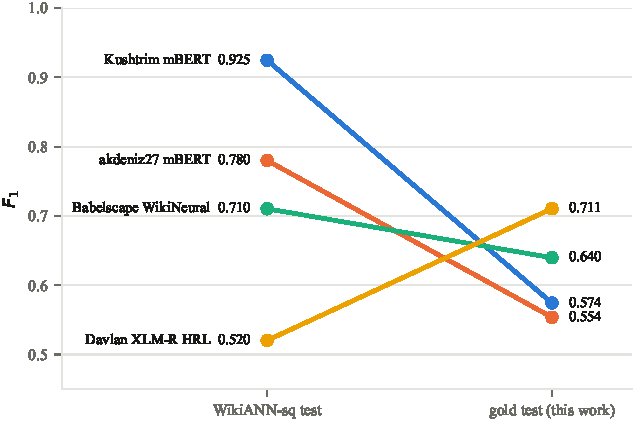
\includegraphics[width=\linewidth]{images/fig_transfer}
\caption{The same four checkpoints, the same scoring routine, two benchmarks. Rank on
WikiANN-sq does not predict rank on hand-verified Albanian prose; Spearman's
$\rho = -0.80$.}
\label{fig:transfer}
\end{figure}

The best model on WikiANN-sq is the third-best here, losing 0.351 $F_1$; the worst model on
WikiANN-sq is the best here, gaining 0.191. Spearman's rank correlation between the two
orderings is $-0.80$, close to a perfect inversion. Every pairwise gap on the gold split is significant under a paired bootstrap except
Kushtrim against akdeniz27 ($p = 0.345$), so the new ordering is not an artefact of the
test sample.

This is the central result of the report, and it is worth stating carefully. It does not
show that the Albanian-specific checkpoints are bad models, nor that their published
numbers are wrong: those numbers are reproducible, and Section~\ref{sec:results:baselines}
reproduces them. It shows that a WikiANN-sq score does not predict performance on
full-length Albanian prose --- in this comparison it predicts it \emph{backwards}. A
practitioner choosing an Albanian NER model by its WikiANN score would have selected the
worst of the four available options for running text.

The mechanism is visible in how the corpora differ. The two mBERT checkpoints were trained
on WikiANN-sq, whose median sentence is 6 tokens and which contains fragments and residual
markup (Section~\ref{sec:results:corpus}). They are strongest on text of that shape and
degrade on the 20-token sentences here. Davlan XLM-R HRL was trained on high-resource
languages and applied to Albanian zero-shot, so it never fitted WikiANN-sq's idiosyncrasies
and transfers to ordinary prose more evenly.

It would overstate the evidence to conclude from this that training on WikiANN-sq damages a
model, because the mismatch runs both ways. A model fine-tuned on the gold corpus here
scores 0.548 $\pm$ 0.020 on WikiANN-sq test, against 0.707 $\pm$ 0.027 on its own test split
(Section~\ref{sec:results:gold-finetune}). Set beside Kushtrim's 0.574 on the gold split,
the picture is symmetric: each model reaches roughly 0.55--0.57 on the corpus it was not
trained on, whichever direction the move is made.

One explanation can be ruled out. The two corpora might simply disagree about where entities
end, in which case the cross-benchmark drop would be a scoring artefact rather than a
modelling result. They do not: mean entity length is 2.30 tokens in WikiANN-sq test against
1.93 under the full-span convention used here (1.68 under the head convention). WikiANN's
spans are the \emph{wider} of the two, so a model predicting full spans is not being
penalised for over-reaching, and the head convention would fare worse still.

What the evidence supports is narrower than a claim about damage, and more useful. The two
benchmarks measure different things, neither substitutes for the other, and a WikiANN-sq
score does not order models by their performance on running text --- in this comparison it
orders them almost exactly backwards. Since applications process running text, that is the
setting an evaluation set has to represent, and none existed for Albanian.

\subsection{Fine-tuning on the annotated corpus}
\label{sec:results:gold-finetune}

Fine-tuning \texttt{xlm-roberta-base} on 483 gold training sentences reaches
$F_1 = 0.709 \pm 0.028$ across three seeds (Table~\ref{tab:gold-finetune},
Appendix~\ref{app:finetune}), against 0.711
for the best zero-shot checkpoint. A paired bootstrap gives a difference of $+0.012$ with a
95\% interval of $[-0.034, +0.055]$ and $p = 0.590$: the two are indistinguishable.



The same three models were also scored on WikiANN-sq test, giving
$F_1 = 0.548 \pm 0.020$. That number belongs with the transfer discussion in
Section~\ref{sec:results:transfer}: it establishes that the domain gap is symmetric rather
than a one-way deficiency of the silver corpus. Note that it is the more precisely measured
of the two figures, since WikiANN-sq test has 1\,000 sentences against the gold split's 201.

Three observations, none of them flattering, all of them worth reporting.

First, 483 training sentences do not beat zero-shot cross-lingual transfer. This is a
statement about corpus size rather than about the pipeline, which reaches parity with
published work when given WikiANN's 5\,000 sentences
(Section~\ref{sec:results:validation}).

Second, \texttt{ORG} is much the weakest class at $F_1 = 0.530$, against 0.855 for
\texttt{PER}. The corpus contains 192 \texttt{ORG} entities in total, so this is likely a
data-quantity problem before it is a modelling one --- and it matches \texttt{ORG} being
hardest for every published checkpoint (Section~\ref{sec:results:errors}).

Third, seed 3 scored 0.677 on test while achieving the second-highest dev score of the
three. With 121 development sentences, epoch selection is barely better than chance, and
the $\pm 0.028$ figure should be read as a lower bound on true run-to-run variance rather
than a tight estimate. Combined with the $\pm 0.06$ confidence interval that 201 test
sentences afford, this corpus can currently resolve differences of roughly 0.12 and no
finer. That bound, rather than any single score, is what the present corpus size buys.

\subsection{Fine-tuning: pipeline validation}
\label{sec:results:validation}

Before applying the training pipeline to the annotated data, it was validated on
WikiANN-sq. A fine-tuned \texttt{xlm-roberta-base} reached $F_1 = 0.928$ on the WikiANN
test split, against 0.925 for the published Kushtrim checkpoint. A paired bootstrap gives a
difference of $+0.003$ with a 95\% confidence interval of $[-0.012, +0.018]$ and $p =
0.691$: the two are statistically indistinguishable.

This is reported not as a contribution but as a control. It establishes that the training
configuration reaches parity with published work on the standard benchmark, so differences
observed later on the annotated corpus are attributable to the data rather than to the
training setup.

\subsection{Annotation}
\label{sec:results:annotation}

%% Written from the campaign as of 2026-09-04: 10 of 12 batches complete. Batches 02 and
%% 07 are still outstanding; update the counts here if they land before submission.

Ten annotators completed 1\,000 annotations covering 820 distinct sentences
(Table~\ref{tab:corpus-stats}). Each batch embedded the same 20 shared sentences, so those
20 carry an annotation from every annotator while the remaining 800 carry one each.

\begin{table}[htbp]
\centering
\caption{The annotated corpus. Head counts entities whose proper-name core is narrower
than the full span --- the cases the dual-boundary convention exists for.}
\label{tab:corpus-stats}
\begin{tabular}{lr}
\toprule
Sentences & 820 \\
Annotations & 1\,000 \\
Annotators & 10 \\
Entities & 1\,207 \\
\quad PER / ORG / LOC & 241 / 192 / 774 \\
Sentences with no entity & 261 \\
Entities where head $\neq$ full span & 183 (15.2\%) \\
Median sentence length & 19 tokens \\
Flagged junk by majority & 15 \\
\bottomrule
\end{tabular}
\end{table}

\paragraph{Inter-annotator agreement.}
Over the 20 shared sentences and all ten annotators, Fleiss' $\kappa$ is 0.829 under the
full-span convention and 0.760 under the head convention; mean pairwise span-level $F_1$ is
0.757 and 0.714. The ordering is expected and informative: the head convention asks
annotators to locate the proper-name core inside a phrase, which is precisely the judgement
Albanian's \emph{X i Y} construction makes ambiguous, so agreement falls when they are
asked to make it. That gap is the empirical case for recording both boundaries rather than
legislating one.

The two measures should be read together. $\kappa$ near 0.83 looks strong, but it is
computed over tokens of which the overwhelming majority are \texttt{O}, where agreement is
trivial. Span-level $F_1$ of 0.757 is the more honest figure, and it says that two
annotators picked from this pool agree on roughly three of four entity spans exactly.
Junk-flag agreement is much weaker ($\kappa = 0.43$): one shared sentence was flagged by
someone and none by everyone, so what counts as unusable text is the least standardised
judgement in the protocol.

\paragraph{The assistance experiment.}
The shared sentences were annotated by five annotators with the model's suggestions visible
and five without, which lets the anchoring question be answered directly rather than
assumed. Agreement is far higher in the assisted condition (Table~\ref{tab:assistance}).

\begin{table}[htbp]
\centering
\caption{Agreement within each condition, over the same 20 shared sentences and five
annotators per condition.}
\label{tab:assistance}
\begin{tabular}{lcccc}
\toprule
& \multicolumn{2}{c}{Fleiss' $\kappa$} & \multicolumn{2}{c}{Pairwise span $F_1$} \\
\cmidrule(lr){2-3}\cmidrule(lr){4-5}
Condition & full & head & full & head \\
\midrule
Assisted & 0.940 & 0.925 & 0.890 & 0.887 \\
From scratch & 0.759 & 0.664 & 0.711 & 0.640 \\
\bottomrule
\end{tabular}
\end{table}

Higher agreement is not the same as higher quality, and the direction of the second
measurement shows why. Scoring each annotator against the model's own pre-labels,
assisted annotators match it at $F_1 = 0.900$ against 0.679 for those working from scratch
(0.913 against 0.645 under the head convention). The two groups do not overlap: the lowest
assisted annotator (0.871) still matches the model more closely than the highest scratch
annotator (0.754). An exact permutation test over all 252 possible splits of ten annotators
into two groups of five gives $p = 0.004$ one-tailed --- the smallest value this design can
produce.

The assisted annotators therefore agree with each other more because they are agreeing with
the model, which is anchoring rather than accuracy. Their errors are correlated by
construction, and a corpus built this way would be evaluated against a standard the model
partly wrote. This is a concrete argument for the from-scratch condition being retained in
the final corpus rather than treated as a control that could be dropped once assistance
proved faster.

\paragraph{Time.}
Assistance did not measurably reduce annotation time. Median time per sentence was 9.6\,s
assisted against 14.3\,s from scratch, but that comparison treats 1\,000 sentences as
independent when the annotator is the real unit: per-annotator medians overlap heavily
(5.6--22.9\,s assisted, 9.4--29.4\,s from scratch), and an exact permutation test on them
gives $p = 0.15$. The apparent 32\% speed-up does not survive being tested at the right
level of aggregation.

Taken together the two results are unfavourable to LLM pre-annotation as used here: it
measurably changed what annotators produced, and did not measurably speed them up.

\subsection{Error analysis}
\label{sec:results:errors}

An $F_1$ score says a model is wrong without saying how. Classifying every mismatch into
four categories --- a gold entity with no overlapping prediction (\emph{missed}), a
prediction overlapping no gold entity (\emph{spurious}), the same token extent with the
wrong type (\emph{type}), and overlapping extents that do not match exactly
(\emph{boundary}) --- separates failures that annotation guidelines can address from
failures that are modelling problems (Figure~\ref{fig:errors}, Appendix~\ref{app:errors}).



Three findings stand out.

\emph{Boundary errors are overwhelmingly under-extensions.} Across every model, a span
that is wrong at its edges is far more often too short than too long --- 150 against 5 for
akdeniz27, 116 against 7 for Babelscape, 153 against 1 for Davlan. Models truncate
multi-token entities rather than over-reaching. This is directly relevant to the
annotation design: Albanian's \emph{X i Y} construction produces exactly the multi-token
spans that are being cut short, which is part of why the boundary convention was recorded
twice rather than fixed in advance (Section~\ref{sec:method:annotation}).

\emph{The reproducibility gap is a boundary problem, not a recall problem.} The two
mBERT checkpoints nominally trained on the same data differ by 0.145 $F_1$, and the error
profiles show why: 56\% of akdeniz27's errors are boundary errors against 21\% for
Kushtrim. The weaker model is not failing to find entities so much as failing to delimit
them.

\emph{ORG is confused with LOC, in that direction.} ORG$\rightarrow$LOC is the most
common type confusion for four of the five models. This is consistent with the class being
hardest for every model in Table~\ref{tab:baselines}, and with the Albanian pattern in
which institutions are named after places --- a distinction the annotation guidelines had
to legislate explicitly.
